\documentclass[dvipdfmx]{beamer}
\usepackage{tutorial}

\title{計算機実験(L7) --- 最適化問題・スーパーコンピューターと計算物理}
\date{2016/06/29}

\begin{document}

\begin{frame}
  \titlepage
  \tableofcontents
\end{frame}

\section{最適化問題}

\begin{frame}[t,fragile]{最適化問題}
  \begin{itemize}
    %\setlength{\itemsep}{1em}
  \item 目的関数$f(x)$の最小値(あるいは最大値)とその場所を求めたい
    \begin{itemize}
    \item 連続最適化問題
    \item 離散最適化(組み合わせ最適化)問題 $\Leftarrow$ 難しい
    \end{itemize}
  \item 真の(大局的な)最小値(最大値)を求めるのは難しい
  \item 一般的には極値を求めることしかできない
  \item 多次元では極小を囲い込むことができない
  \item 導関数を使う方法: ニュートン法、最急降下法、共役勾配法、準ニュートン法
  \item 使わない方法: 囲い込み法、Nelder-Meadの滑降シンプレックス法、シミュレーテッド・アニーリング
  \end{itemize}
\end{frame}

\section{最急降下法と勾配降下法}

\begin{frame}[t,fragile]{最急降下法(steepest descent)}
  \begin{itemize}
    \setlength{\itemsep}{1em}
  \item 関数の微分の情報を使う
  \item 現在の点$\bf x$における勾配を計算
    \[
    -\nabla f|_i = -\frac{\partial f}{\partial x_i}
    \]
  \item 坂を下る方向にそって、一次元最適化
  \item 動いた先の勾配の方向でさらに最適化を繰り返す
  \item 関数値は単調減少 $\Rightarrow$ 極小値に収束
  \end{itemize}
\end{frame}

\begin{frame}[t,fragile]{勾配降下法(gradient descent)}
  \begin{itemize}
    \setlength{\itemsep}{1em}
  \item 勾配方向に一次元最適化を行うかわりに、あらかじめ決めた一定量($\epsilon$)だけ坂を下る
    \[
    x_{n+1} = x_n - \epsilon \, \nabla f
    \]
  \item あらかじめ最適な$\epsilon$を知るのは困難
  \item 機械学習の分野では、(なぜか) $\epsilon=0.1$が良いとされている
  \item この方法を「最急降下法」、一次元最適化を行う勾配法を「最適降下法(optimum descent)」と呼ぶ場合も
  \item c.f.) 確率的勾配降下法(stochastic gradient descent)
  \end{itemize}
\end{frame}

\begin{frame}[t,fragile]{制約条件付きの場合}
  \begin{itemize}
    % \setlength{\itemsep}{1em}
  \item 目的関数: $f(x)$
  \item 制約条件:
    \begin{itemize}
    \item $g_i(x) = 0$ \ ($i=1,\cdots,m$) \ (等式制約条件)
    \item $h_j(x) \ge 0$ \ ($j=1,\cdots,n$) \ (不等式制約条件)
    \end{itemize}
  \item 等式制約条件の付いている場合: Lagrangeの未定乗数法
    \[
    L(x,\lambda_1,\cdots,\lambda_m)=f(x)+\sum_i \lambda_i g_i(x)
    \]
    を考え、$x,\lambda_1,\cdots,\lambda_m$の微分が零となる点を探す
  \item 不等式制約条件の付いている場合: c.f. 線形計画法, ペナルティ関数法
  \end{itemize}
\end{frame}

\begin{frame}[t,fragile]{細長い谷の場合}
  \vspace*{1em}
  \hspace*{1em}\resizebox{1\textwidth}{!}{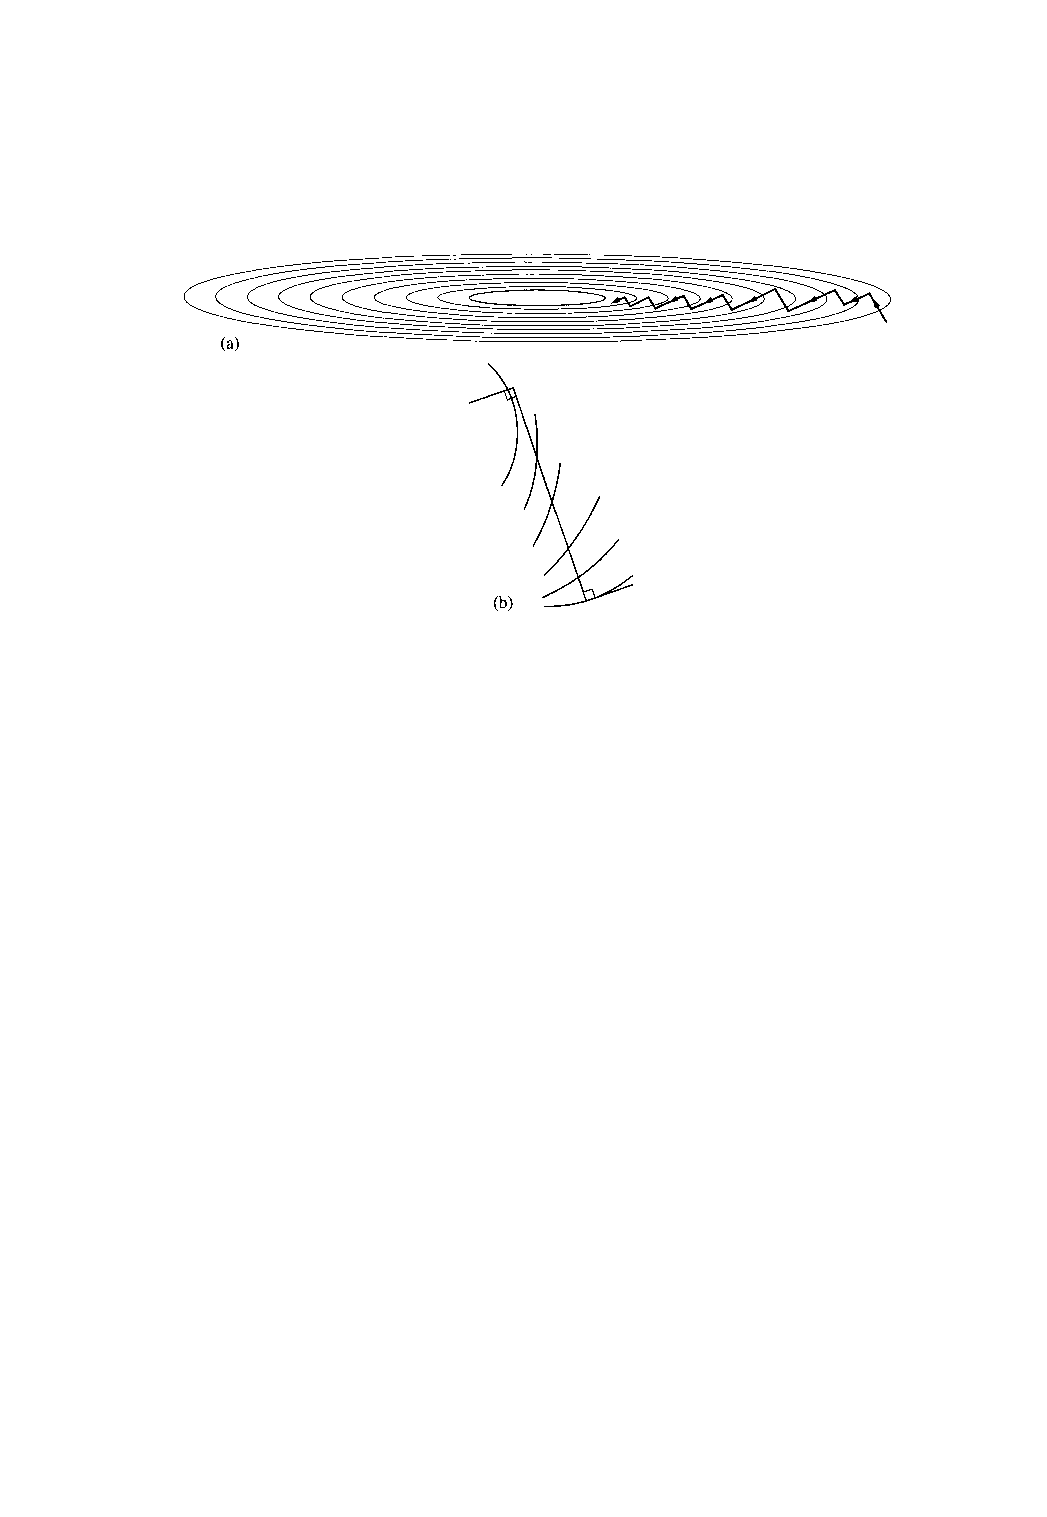
\includegraphics{image/steepest-descent.pdf}}

  \vspace*{-2em}
  \hspace*{20em}{\footnotesize(Press et al 1988)}
\end{frame}

\section{最適化手法の比較}

\begin{frame}[t,fragile]{例題 (二次元の最適化)}
  \begin{center}
    \resizebox{.9\textwidth}{!}{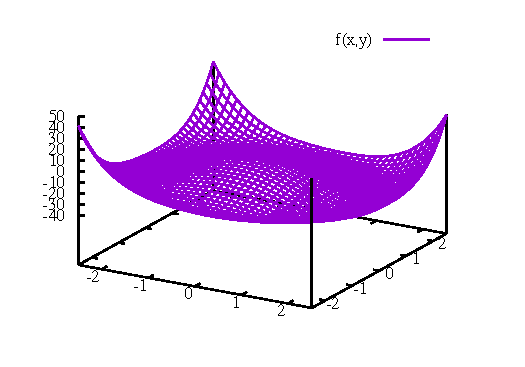
\includegraphics{image/func_2d.pdf}}
  \end{center}
\end{frame}

\begin{frame}[t,fragile]{様々な最適化手法の比較 (1/4)}
  \begin{center}
    \resizebox{.9\textwidth}{!}{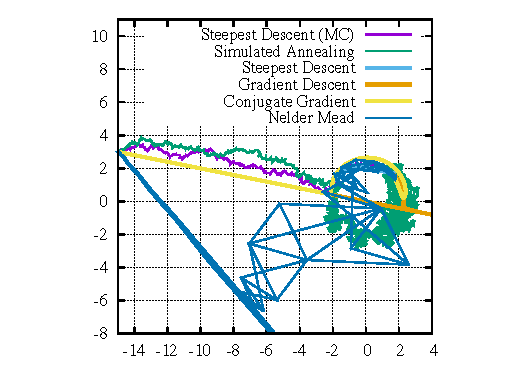
\includegraphics{image/optimization.pdf}}
  \end{center}
\end{frame}

\begin{frame}[t,fragile]{様々な最適化手法の比較 (2/4)}
  \begin{center}
    \resizebox{.9\textwidth}{!}{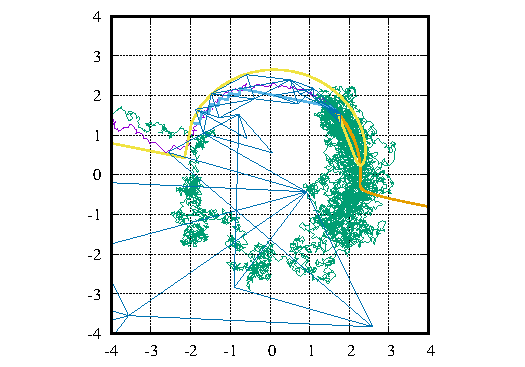
\includegraphics{image/optimization2.pdf}}
  \end{center}
\end{frame}

\begin{frame}[t,fragile]{様々な最適化手法の比較 (3/4)}
  \begin{center}
    \resizebox{.9\textwidth}{!}{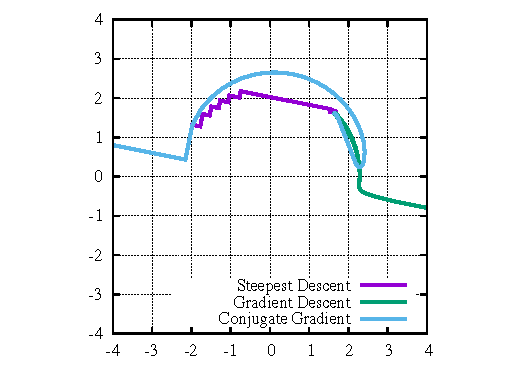
\includegraphics{image/optimization3.pdf}}
  \end{center}
\end{frame}

\begin{frame}[t,fragile]{様々な最適化手法の比較 (4/4)}
  \begin{center}
    \resizebox{.9\textwidth}{!}{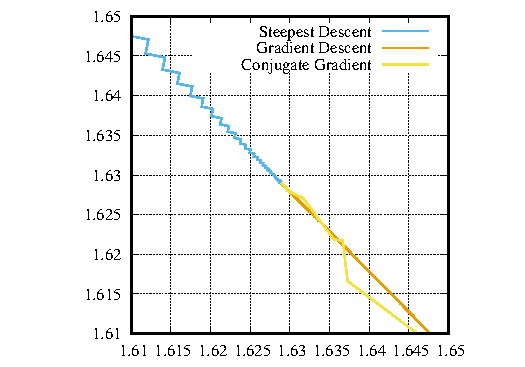
\includegraphics{image/optimization4.pdf}}
  \end{center}
\end{frame}

\section{スーパーコンピューターと計算物理}

\begin{frame}[t,fragile]{計算機の進化}
  \begin{itemize}
    \setlength{\itemsep}{1em}
  \item 計算機の性能は指数関数的に伸び続けている
    \begin{itemize}
    \item 1年で1.9倍 ⇒ 4年で10倍 ⇒ 過去70年間で100兆倍
    \item 世界初のスパコンCray-1 (1976年)の演算性能 約160MFlops
    \item iPhone6 (2014年)の演算性能 約900MFlops
    \item 2020年代初頭には、1EFlops (エクサフロップス)へ
    \end{itemize}
  \item 現代のスーパーコンピュータは全て
    \begin{itemize}
      \item 並列コンピュータ (CPU数 1,000〜100,000)
      \item マルチコア or メニーコア (CPUあたりのコア数 8 〜 1,000)
      \item 多層にわたる階層構造
      \item 演算に比べて、データを移動するコストの方が高い
    \end{itemize}
  \end{itemize}
\end{frame}

\section{並列計算とは}

\begin{frame}[t,fragile]{Richardson's Forecast Factory (1922)}
  \resizebox{.8\textwidth}{!}{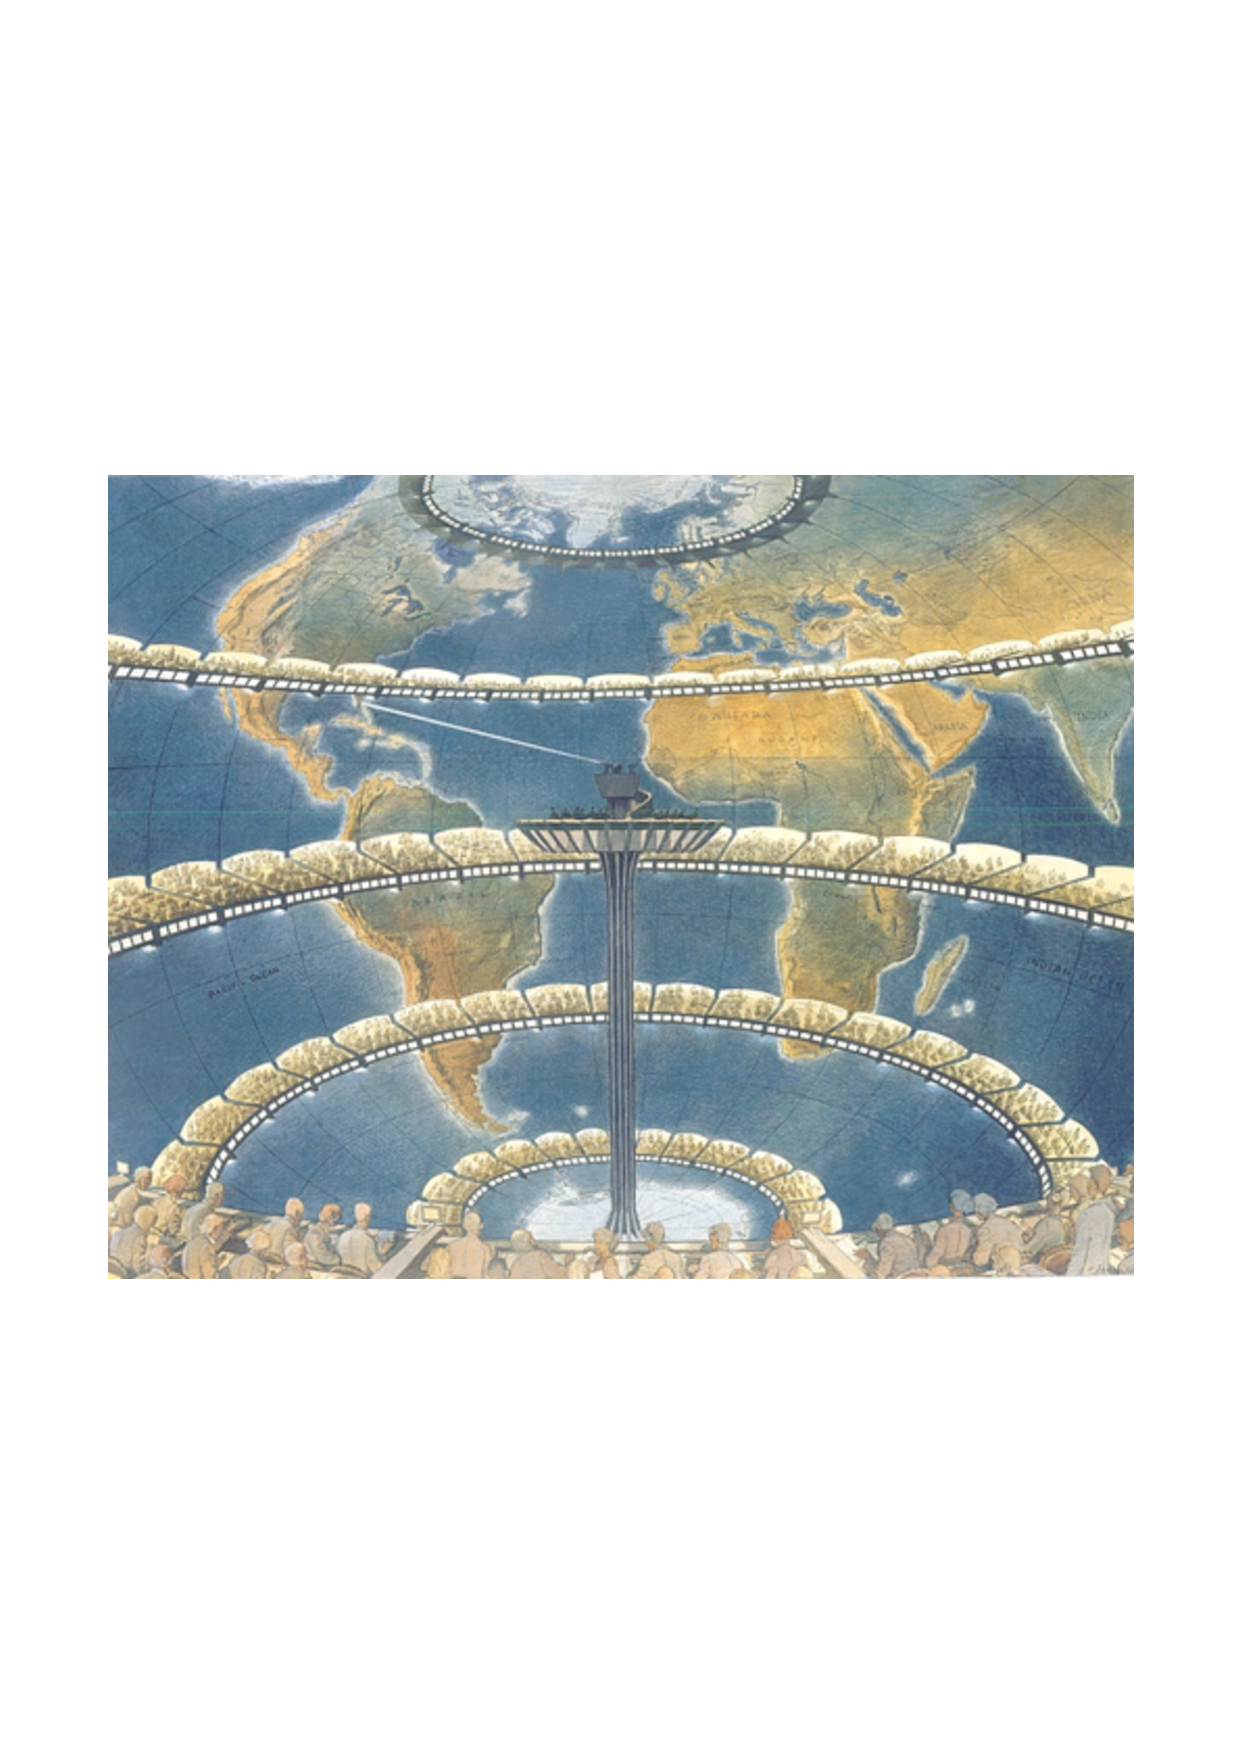
\includegraphics{image/SchuitenHD3.pdf}}
\end{frame}

\begin{frame}[t,fragile]{並列化とは何か}
  \begin{itemize}
    \setlength{\itemsep}{1em}
  \item 目的: シミュレーションをできる限り「短時間」で終了させる
    \begin{itemize}
      \item たとえ総CPU時間が伸びても「ターンアラウンド時間」を短かくしたい
      \item 一台のパソコンでは100年かかる計算を学位論文に間に合わせたい
      \item 今の100倍の精度の計算を同じ「実時間」で実行したい
    \end{itemize}
  \item 並列化とは
    \begin{enumerate}
    \item CPUの行なうべき仕事を複数の小さな仕事に分割
    \item それらを複数のCPUで同時実行
    \end{enumerate}
  \item うまく並列化を行なうために必要なこと
    \begin{enumerate}
    \item プログラムのどの部分をどのように並列化すればより効果的かを理解する
    \item 並列化を実装するにはどのようにプログラムを書けば良いかを理解する
    \end{enumerate}
  \end{itemize}
\end{frame}

\begin{frame}[t,fragile]{並列計算の原理}
  \begin{itemize}
    %\setlength{\itemsep}{1em}
  \item ノードは、互いに必要な情報を交換しながら、それぞれ異なる処理をしなければならない
  \item ノード毎に異なる指示(= プログラム)を与えるのは大変 (特にノード数が何万もの場合)
  \item 一つのプログラムでノード(ランクとも呼ばれる)毎に異なる指示を与えたい

    ⇒ SPMD (Single Program, Multiple Data streams)

    \resizebox{.9\textwidth}{!}{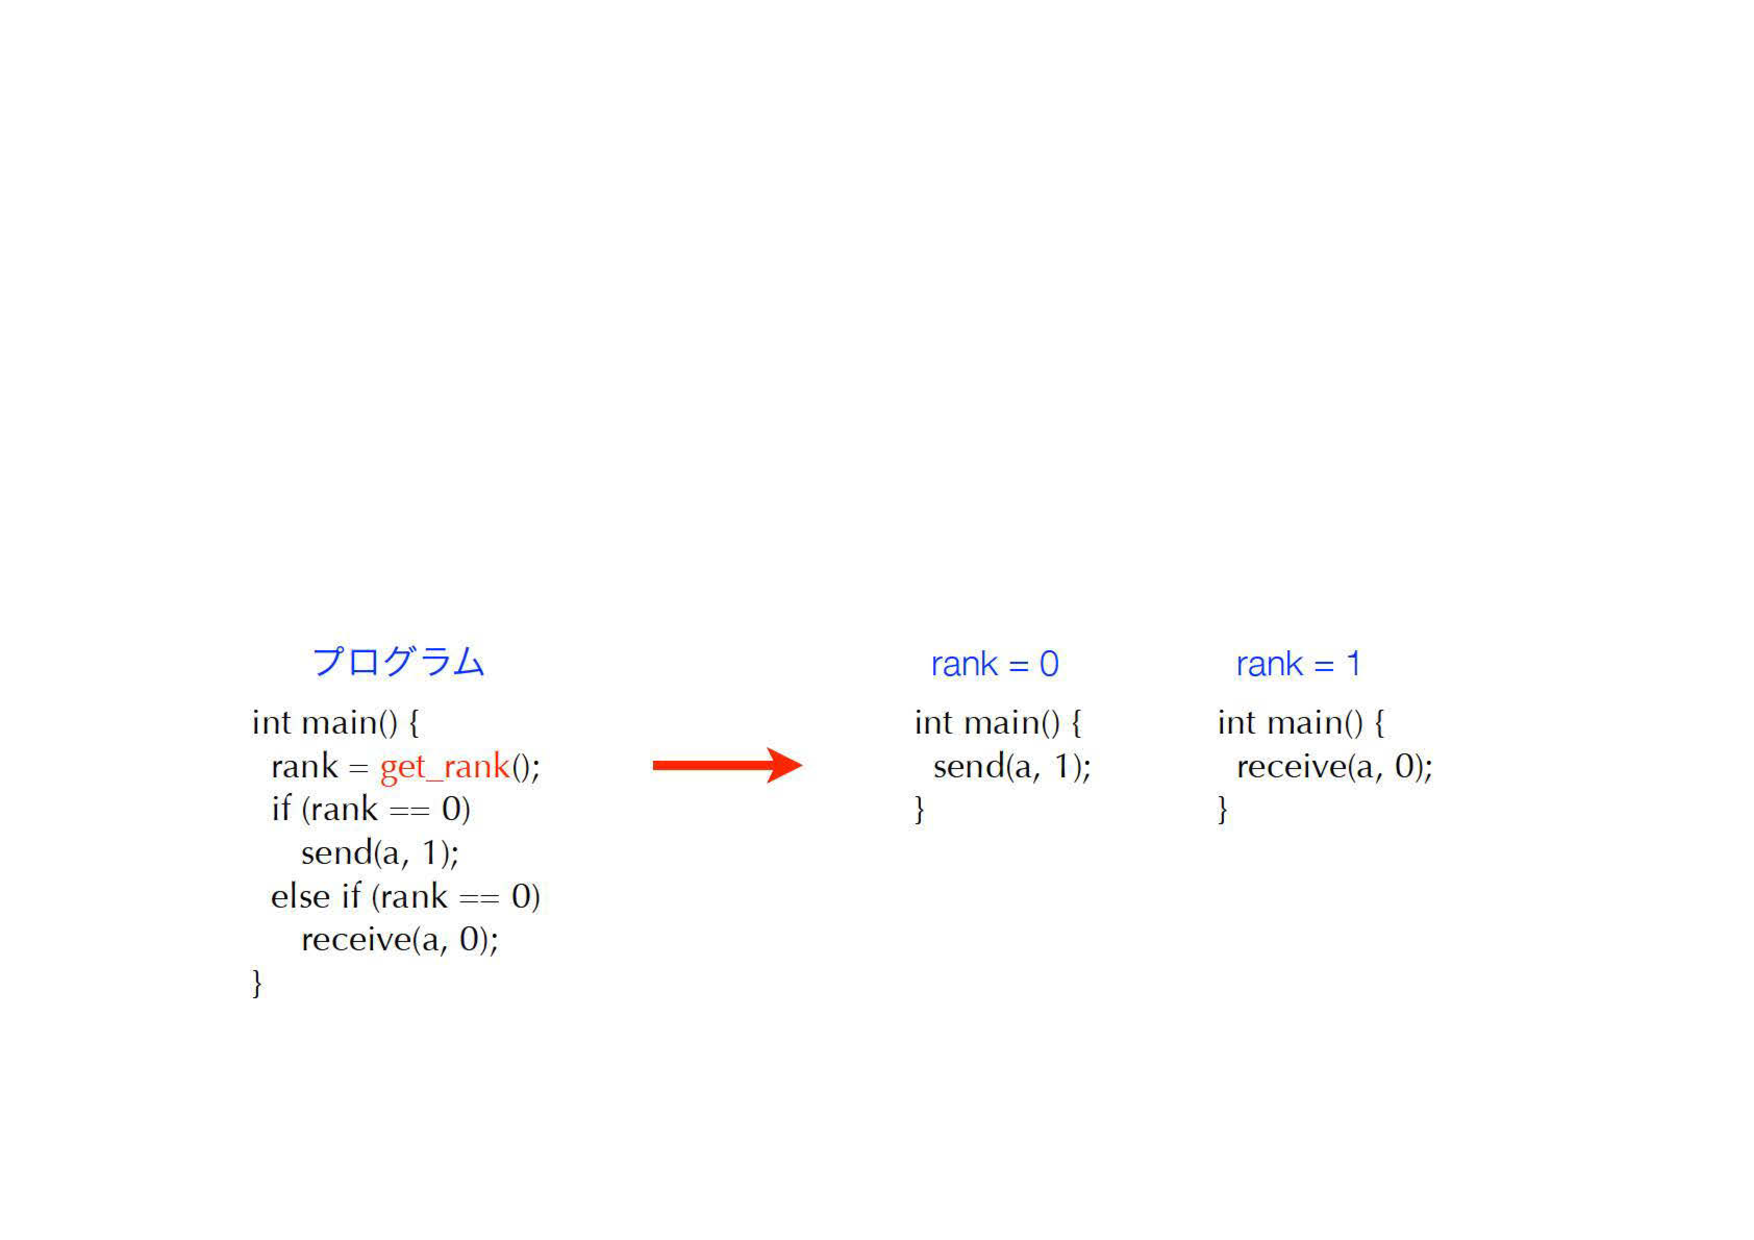
\includegraphics{image/spmd.pdf}}
  \end{itemize}
\end{frame}

\begin{frame}[t,fragile]{アムダール(Amdahl)の法則}
  \begin{itemize}
    \setlength{\itemsep}{1em}
  \item 並列化による全体の性能向上率
    \[
    P = \frac{1}{X+(1-X)/n}
    \]
    $X$: 並列化されていない部分の実行時間の割合, $n$: ノード数
  \item $X$を限りなく零にしないと高並列ではすぐに性能が頭打ちに
  \end{itemize}
  \vspace*{-0em}\hspace*{1em}\resizebox{0.5\textwidth}{!}{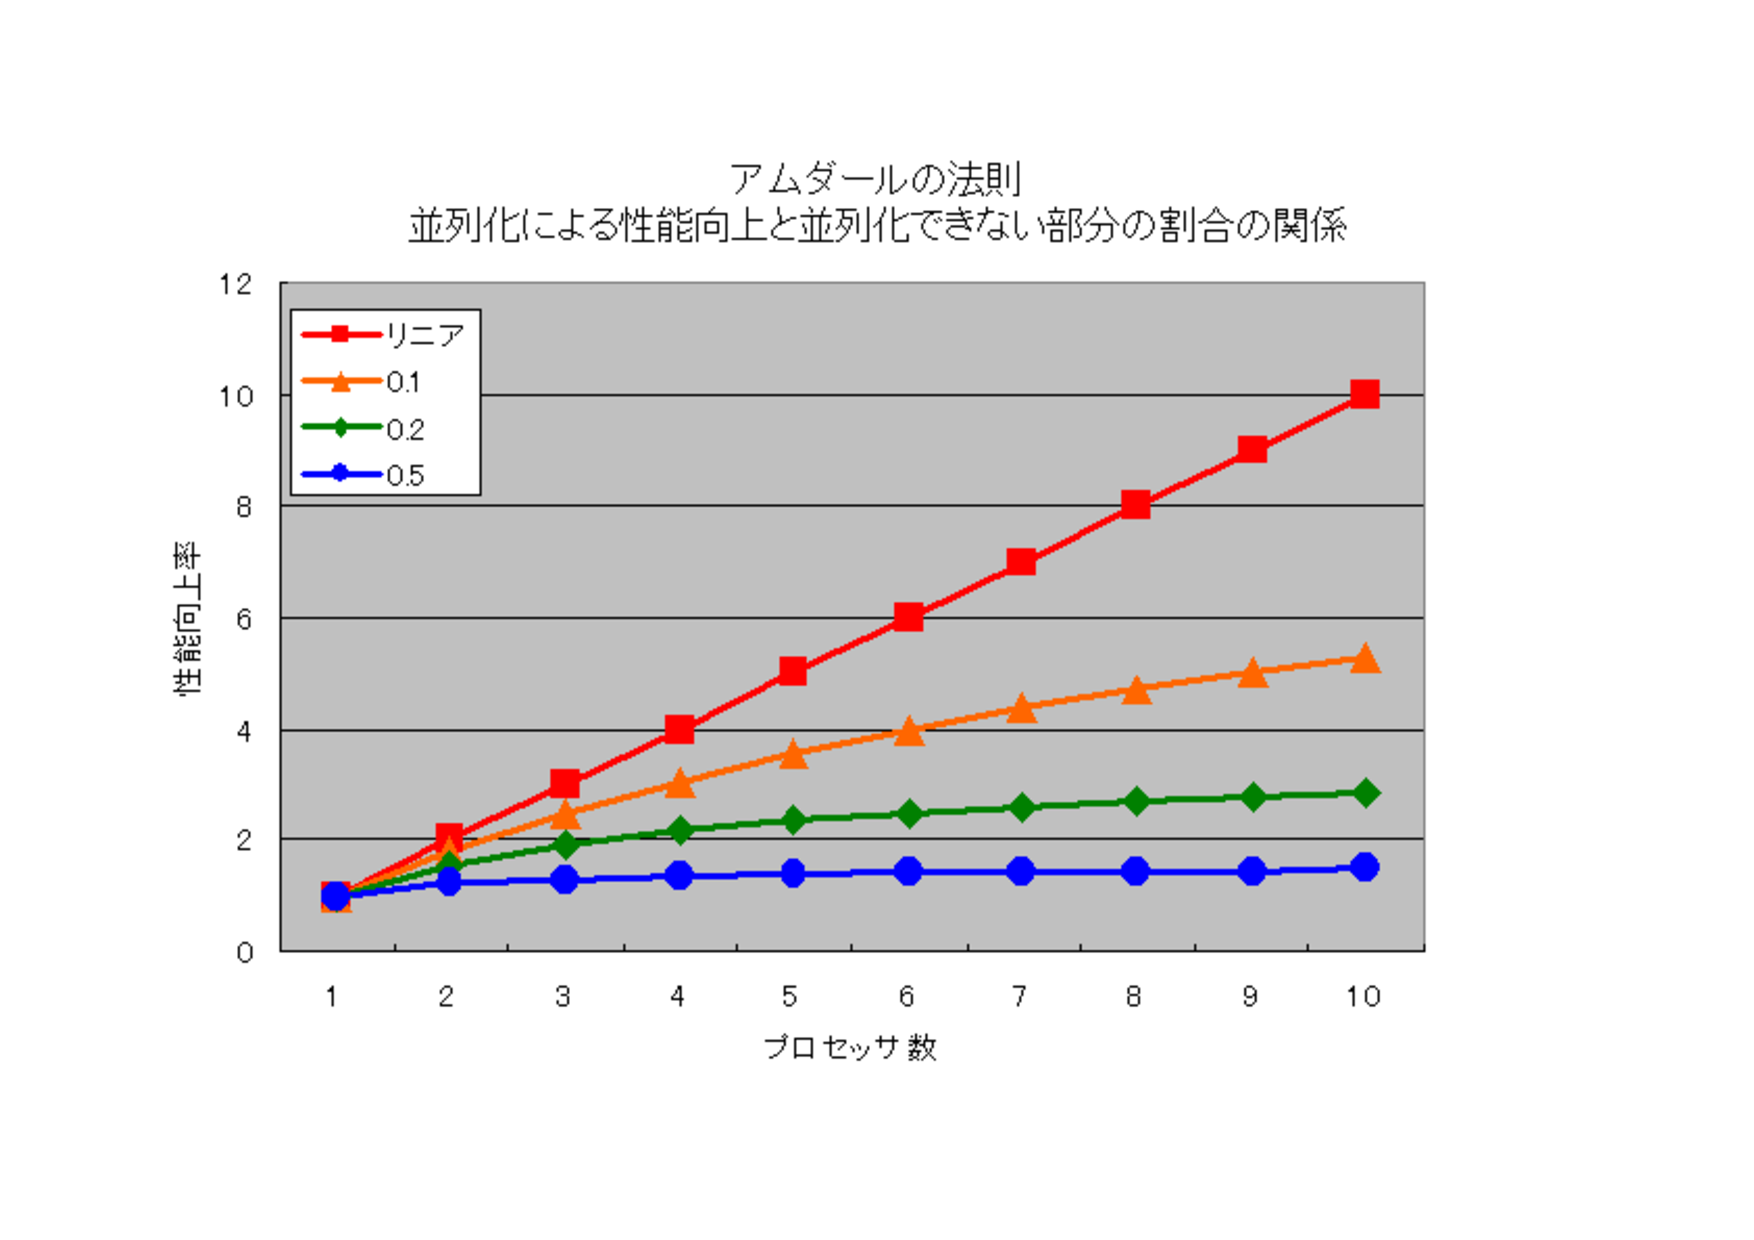
\includegraphics{image/Amdahl_law2.pdf}}
\end{frame}

\section{バッチキューシステム}

\begin{frame}[t,fragile]{バッチキューシステム}
  \begin{itemize}
    \setlength{\itemsep}{1em}
  \item 実習用計算機 photon
    \begin{itemize}
    \item ログインノード(2CPU, 12コア)+計算ノード(64CPU, 256コア)からなる「クラスタワークステーション」(並列計算機の一種)
    \item 普段{\tt ssh}して作業しているのはログインノード
    \end{itemize}
  \item バッチーキューシステム
    \begin{itemize}
    \item 長い(大きな)計算は計算ノードを使う
    \item 多数の計算ノードの割り振りを手でやるのは非効率的
    \item バッチキューシステムを使って、「ジョブ」を投入する
    \end{itemize}
  \item 詳しい説明は「システム利用マニュアル」({\tt ssh}ログイン時に表示されるメッセージ参照)を見ること
  \item photon は卒業まで継続して利用可 (希望すれば大学院でも)
  \end{itemize}
\end{frame}


\section{}

\begin{frame}[t,fragile]{実習・講義予定}
  \begin{itemize}
    \setlength{\itemsep}{1em}
  \item 実習 EX6
    \begin{itemize}
    \item モンテカルロ法
    \item 最適化
    \item レポートNo.3: 締切7/29(金)
    \end{itemize}
  \item 7/13 グループワーク発表会
    \begin{itemize}
    \item タイトル・ライトニングトーク用スライド(PPT・1枚): 締切7/12(火)
    \item ポスター掲示(1220室前のロビー): 7/13(水) 10:15-10:25
    \item ライトニングトーク: 10:25-11:00 (各グループ2分以内)
    \item ポスターセッション: 11:00-12:10
    \item グルプーレポート: ポスター(を修正したもの)を提出。締切7/15(金)
    \item 発表会に関する連絡事項等はITC-LMSに掲載するので、適宜確認すること
    \end{itemize}
  \end{itemize}
\end{frame}

\end{document}
